\documentclass[12pt,a4paper]{article}
\usepackage[utf8]{inputenc}
\usepackage[bottom=2cm,top=2cm,left=2cm,right=2cm]{geometry}
\usepackage{a4wide,amssymb,epsfig,latexsym,multicol,array,hhline,fancyhdr}
\usepackage{booktabs}
\usepackage{amsmath}
\usepackage{lastpage}
\usepackage[lined,boxed,commentsnumbered]{algorithm2e}
\usepackage{enumerate}
\usepackage{color}
\usepackage{graphicx}							% Standard graphics package
\usepackage{array}
\usepackage{tabularx, caption}
\usepackage{multirow}
\usepackage[framemethod=tikz]{mdframed}% For highlighting paragraph backgrounds
\usepackage{multicol}
\usepackage{rotating}
\usepackage{graphics}
\usepackage{setspace}
\usepackage{epsfig}
\usepackage{tikz}
\usepackage{listings}
\usetikzlibrary{arrows,snakes,backgrounds}
\usepackage{hyperref}
\hypersetup{urlcolor=blue,linkcolor=black,citecolor=black,colorlinks=true} 

\everymath{\color{black}}
%\usepackage{fancyhdr}
\setlength{\headheight}{40pt}
\pagestyle{fancy}
\fancyhead{} % clear all header fields
\fancyhead[L]{
 \begin{tabular}{rl}
    \begin{picture}(25,15)(0,0)
    \put(0,-8){
\includegraphics[width=8mm, height=8mm]{imgs/hcmut.png}}
    %\put(0,-8){\epsfig{width=10mm,figure=hcmut.eps}}
   \end{picture}&
	%
\includegraphics[width=8mm, height=8mm]{hcmut.png} & %
	\begin{tabular}{l}
		\textbf{\bf \ttfamily Ho Chi Minh City University of Technology}\\
		\textbf{\bf \ttfamily Faculty of Computer Science \& Engineering}
	\end{tabular} 	
 \end{tabular}
}
\fancyhead[R]{
	\begin{tabular}{l}
		\tiny \bf \\
		\tiny \bf 
	\end{tabular}  }
\fancyfoot{} % clear all footer fields
\fancyfoot[L]{\scriptsize \ttfamily Computer Networks}
\fancyfoot[R]{\scriptsize \ttfamily Page {\thepage}/\pageref{LastPage}}
\renewcommand{\headrulewidth}{0.3pt}
\renewcommand{\footrulewidth}{0.3pt}


%%%
\setcounter{secnumdepth}{4}
\setcounter{tocdepth}{3}
\makeatletter
\newcounter {subsubsubsection}[subsubsection]
\renewcommand\thesubsubsubsection{\thesubsubsection .\@alph\c@subsubsubsection}
\newcommand\subsubsubsection{\@startsection{subsubsubsection}{4}{\z@}%
                                     {-3.25ex\@plus -1ex \@minus -.2ex}%
                                     {1.5ex \@plus .2ex}%
                                     {\normalfont\normalsize\bfseries}}
\newcommand*\l@subsubsubsection{\@dottedtocline{3}{10.0em}{4.1em}}
\newcommand*{\subsubsubsectionmark}[1]{}
\makeatother

\definecolor{dkgreen}{rgb}{0,0.6,0}
\definecolor{gray}{rgb}{0.5,0.5,0.5}
\definecolor{mauve}{rgb}{0.58,0,0.82}

\lstset{frame=tb,
	language=Matlab,
	aboveskip=3mm,
	belowskip=3mm,
	showstringspaces=false,
	columns=flexible,
	basicstyle={\small\ttfamily},
	numbers=none,
	numberstyle=\tiny\color{gray},
	keywordstyle=\color{blue},
	commentstyle=\color{dkgreen},
	stringstyle=\color{mauve},
	breaklines=true,
	breakatwhitespace=true,
	tabsize=3,
	numbers=left,
	stepnumber=1,
	numbersep=1pt,    
	firstnumber=1,
	numberfirstline=true
}

\begin{document}
\begin{titlepage}
\begin{center}
VIETNAME NATIONAL UNIVERSITY HO CHI MINH CITY  \\
HO CHI MINH CITY UNIVERSITY OF TECHNOLOGY\\
FACULTY OF COMPUTER SCIENCE AND ENGINEERING
\end{center}

\vspace{1cm}

\begin{figure}[h!]
\begin{center}

\includegraphics[width=3cm]{imgs/hcmut.png}
\end{center}
\end{figure}

\vspace{1cm}


\begin{center}
\begin{tabular}{c}
	\multicolumn{1}{l}{\textbf{{\Large COMPUTER NETWORKS}}}\\
	~~\\
	\hline
	\\
	\multicolumn{1}{l}{\textbf{{\Large Lab 1}}}\\
	\\
	
	\textbf{{\Huge Behavior of the TCP protocol}}\\
	\\
	\hline
\end{tabular}
\end{center}

\vspace{3cm}

\begin{table}[h]
\begin{tabular}{rrl}
\hspace{5 cm} & GVHD: &Giang Xuan Bui\\
                & Students: & Thang Huu Nguyen - 1713239\\
                % & & Mai Đức Tú - 1513924 \\
                % & & Phồng Quang Tuấn - 1513865\\
                % & & Lê Duy Hiển - 1511057 \\
                % & & Nguyễn Đỗ Đức Anh - 1510062\\
\end{tabular}
\end{table}

\vspace{3cm}

\begin{center}
{\footnotesize Ho Chi Minh City, August 2019}
\end{center}
\end{titlepage}

\newpage

\section{What is the IP address and TCP port number used by the client computer (source) that is transferring the file to \\ gaia.cs.umass.edu? To answer this question, it’s probably easiest to select an HTTP message and explore the details of the TCP packet used to carry this HTTP message, using the “details of the selected packet header window” (refer to Figure 2 in the “Getting Started with Wireshark” Lab if you’re uncertain about the Wireshark windows.}

\begin{figure}[h]
    \centering
    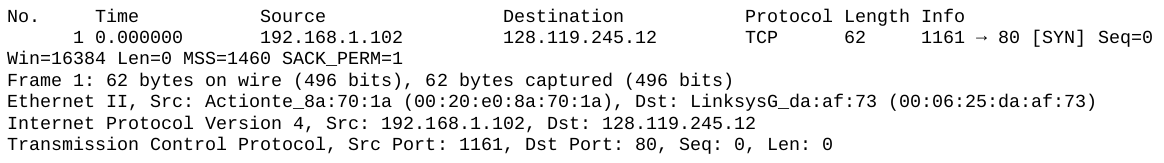
\includegraphics[width=\linewidth]{imgs/Figure1.png}
    \caption{Wireshark captured packet file tcp-ethereal-trace-1}
    \label{fig:tcp-ethereal-trace-1}
\end{figure}

According to Figure 1, the IP address and TCP port number used by the client computer (source) that is transferring the file to gaia.cs.umass.edu are:

\begin{itemize}
    \item IP address: 192.168.1.102
    \item TCP port: 1161
\end{itemize}

\section{What is the IP address of gaia.cs.umass.edu? On what port number is it sending and receiving TCP segments for this connection?}



\section{What is the IP address and TCP port number used by your client computer (source) to transfer the file to gaia.cs.umass.edu?}

\begin{figure}[h]
    \centering
    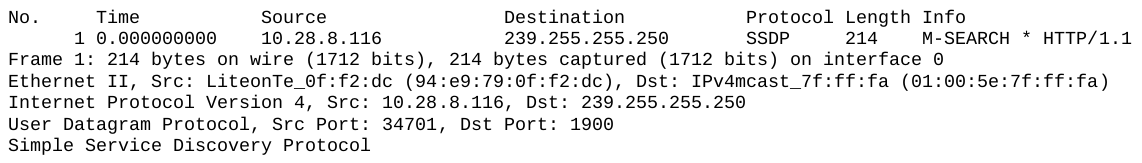
\includegraphics[width=\linewidth]{imgs/Figure2.png}
    \caption{Wireshark captured packet file tcp-personal-trace}
    \label{fig:tcp-personal-trace}
\end{figure}

According to Figure 2, the IP address and TCP port number used by the my computer (source) that is transferring the file to gaia.cs.umass.edu are:

\begin{itemize}
    \item IP address: 10.28.8.116
    \item TCP port: 34701
\end{itemize}

\end{document}
